\chapter{基于乘法器库和强化学习方法的近似逻辑综合研究}

\section{引言}

不同近似乘法器的精度和硬件成本通常不同,单独地看,硬件设计人员可以根据精度需求直接选出库中硬件性能最高的近似乘法器使用。然而,实际情况通常是对某个大型电路挑选最适合的近似乘法器,这里适合的意思是指电路整体的PPA最优。对大型电路来讲,乘法器单元通常作为数据通路的一部分与别的电路耦合在一起,因此大规模电路的性能评估不能只从乘法器单元的硬件开销进行判断,而应该从整体进行分析。

基于第三章和第四章得到的近似乘法器库,面向大规模电路,本章利用强化学习方法对不同乘法器实现的DNN硬件加速器进行了近似逻辑综合的研究。具体来讲,本章首先提出了一个强化学习序列探索框架,能够对大电路进行全面的优化,接着将优化框架和基于数据分布和输入极性得到的DNN近似乘法器库结合起来,研究不同近似乘法器对大规模电路(以DNN硬件加速器为例)带来的影响。

\section{面向大规模电路的强化学习逻辑优化框架}

\subsection{现有序列优化方法存在的问题}

目前已有的序列优化方法\cite{LS:BOiLS,LS:DRiLLS}在针对大规模电路进行探索时迭代速度慢,无法在有限地时间内得到高质量的输出结果,尽管有工作\cite{LS:Bulls-Eye}在基于图神经网络训练一个预测器后利用主动学习的方法能够在较短时间内应用到大网络上,但预测质量往往不如直接探索的方法,同时预测器的搜索空间是预先固定的,无法进行灵活调整。另外,已有的方法都是直接将一个优化序列应用于整个网络,考虑到电路的算术逻辑部分和控制逻辑部分有不同的特性\cite{LS:MIG},网络的不同部分可能适用于不同的序列。

文献\cite{LS:LSOracle}利用超图划分的方法对布尔网络进行分割,并对划分后的子网络选择合适的DAG进行优化,但由于划分后每个子网络的输入信号的到达时间可能不为0,这导致对子网络进行优化时的关键路径可能并不是真实的关键路径,同时超图划分的目标只是最小化割边权重和或子图连通性,并没有考虑节点处于不同子图会带来不同优化效果的影响,且不同DAG的优化引擎质量不一致,这些原因加起来导致合并后的网表经过评估后优势不大。因此需要针对大规模网络提出一个基于高质量划分的序列探索方法,既能充分利用现代CPU架构的多核特性提高探索效率,又能保证合并后优化质量的提升。


\subsection{基于MFFC自适应超图划分的端到端强化学习逻辑优化框架}

\begin{figure}[!htbp]
    \centering
    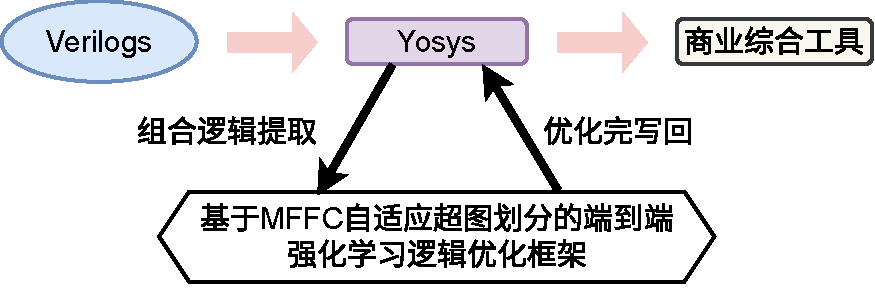
\includegraphics[width=0.8\linewidth]{./figs/LS-MFFC_rl.pdf}
    \caption{本文提出的强化学习逻辑优化框架流程图}
    \label{LS:MFFC_rl}
\end{figure}

本文提出并开源了一个基于MFFC自适应超图划分的端到端强化学习逻辑优化框架,该框架基于Yosys\cite{LS:yosys}和ABC\cite{LS:ABC}实现。首先利用Yosys对电路进行读入和解析,接着将电路中的组合逻辑提取出来。基于文献\cite{Moucheng_Yang}的发现,利用ABC将提取的组合逻辑转换成AIG并“自然划分”,得到一个或多个AIG簇(若AIG簇只有一个,则该AIG簇为原AIG),簇与簇之间互相没有任何连接。对“自然划分”后规模仍然较大的簇,利用MFFC遍历将簇转换成以MFFC为节点的超图。之后利用开源的超图划分工具KaHyPar\cite{KaHyPar}采用多层划分的方法对MFFC超图进行划分,即得到AIG簇的划分。划分完成后,对所有的子电路并行地利用提出的强化学习序列优化方法在给定的时间内进行搜索,利用现代CPU的多核特性,对大网络的不同区域进行充分探索,避免对整个网络直接进行优化带来的局限性,提高探索效率。最后合并所有基于找到的高质量序列进行优化后的子电路,写回到Yosys,和时序逻辑一起输出,由商业综合工具进行评估。基于超过150个电路的商业综合工具的评估结果显示,与ABC resyn2相比,面积延迟积平均提高了5.17\%,整体流程如图\ref{LS:MFFC_rl}所示。

% 主要创新点如下:
% \begin{itemize}
%     \item 提出了一个开源的应用于大型电路的端到端强化学习逻辑优化框架,该框架在对布尔网络进行分割后并行地利用强化学习方法进行序列探索,充分利用现代CPU的多核特性,提高探索效率;
%     \item 与不分割相比,划分后能够对大网络的不同区域进行充分探索,避免了基于整个网络进行优化带来的局限性;
%     \item 基于超过150个电路的商业综合工具的评估结果显示,与ABC resyn2相比,面积延迟积平均提高了5.17\%。
% \end{itemize}

(1)自然划分

本文首先利用Yosys对Verilog进行解析,将电路中的组合逻辑和时序逻辑分开,其中,寄存器的输入会变成组合逻辑的输出,寄存器的输出会变成组合逻辑的输入。之后基于文献\cite{Moucheng_Yang}的发现,将提取出的组合逻辑通过ABC读入,转成AIG,并识别出AIG中所有互相之间没有连接的逻辑簇,按照簇将AIG进行分割,易知切割的边数为0,且分割得到的所有簇的主要输入要么来源于电路的输入、要么来源于寄存器的输出,因此所有簇的输入延迟均为0。

(2)基于MFFC的超图划分

自然划分后,有可能会存在过大的簇,对于过大的簇,首先对所有的节点遍历并计算MFFC,根据\ref{MFFC}的内容可知两个MFFC要么不相交、要么一个包含另一个,当两个MFFC存在包含关系时,保留大的MFFC作为超图中的节点。同时,一个MFFC内节点的值只会影响到该MFFC的根节点和根节点的传递扇出,因此与直接对簇进行划分相比,MFFC超图的出现相当于在划分前将一些应该一起优化的AIG节点捆绑在一起,减少文献\cite{LS:LSOracle}中直接对AIG进行划分带来的缺点。
MFFC超图形成后,对其采用开源的超图划分工具\cite{KaHyPar}进行分割,为了保证分割后每个子图的AIG规模大致相等,MFFC超图中每个节点都有一个权重值,大小为该MFFC的节点数。

(3)提出的强化学习方法

DRiLLS\cite{LS:DRiLLS}在序列探索过程中每次运行一个优化命令都需要保存一个中间文件,效率较低。本文提出并开源了一个新的强化学习逻辑综合方法,该方法基于OpenAI Gym\cite{AI:gym}和Stable Baselines3\cite{AI:stable-baselines3}实现,支持ABC\cite{LS:ABC}、Cirkit\cite{LS:cirkit}、iMAP\cite{LS:iMAP}三个学术界主流的逻辑综合工具,能够完成以逻辑优化、LUT映射、ASIC映射为目标的序列探索任务。

\subsection{实验结果}

对来自OPDB\cite{LS:OPDB}、VTR\cite{FPGA:vtr8}、Koios\cite{FPGA:Koios}、EPFL\cite{LS:EPFL_benchs_iwls,LS:EPFL_benchs_github}、IWLS05\cite{LS:iwls05}、QUIP\cite{LS:quip}等超过150个不同规模的电路进行广泛测试,对提取的组合逻辑网表分别用ABC resyn2、BOiLS\cite{LS:BOiLS}、DRiLLS\cite{LS:DRiLLS}、LSOracle\cite{LS:LSOracle}、以及本文提出的方法在Intel Xeon处理器上利用200个CPU核进行优化,其中BOiLS和DRiLLS使用单线程运行,运行时间由下式确定:
\begin{equation}
    runtime = \lceil \frac{N_{p}}{200} \rceil * 2 h
\end{equation}
其中$N_{p}$代表根据本文提出的方法进行“自然划分”和MFFC超图划分后所有的子电路的总数,$\lceil \ \rceil$表示向上取整。
优化完成后和时序逻辑合并输出,利用Synopsys Design Compiler (DC) S-2021.06-SP5在一个开源的7nm工艺库\cite{ASAP7_github}进行综合,获得面积延迟积(Area Delay Product, ADP)进行比较。为了避免DC的优化对结果带来影响,将电路的时钟频率约束设为0,同时最小化面积(set\_max\_area 0),并使用“compile”命令进行映射。
注意本文并没有考虑划分消耗的时间,对于一个拥有百万个AIG节点的组合逻辑网络来说,“自然划分”和MFFC超图划分所花费的时间总共在10h左右。

\begin{table*}[!htb]
    % \renewcommand{\arraystretch}{1.4}
    % \setlength\tabcolsep{3.76pt}
    \caption{基于不同方法得到的面积、延迟和ADP的平均百分比提升}
    \begin{center}
    \scalebox{0.9}{
        \begin{tabular}{|c|c|c|c|c|c|}
        \hline
        最大的$n$个电路 &  & LSOracle\cite{LS:LSOracle} & BOiLS\cite{LS:BOiLS} & DRiLLS\cite{LS:DRiLLS} & 本文的方法 \\
        \hline
        \multirow{3}{*}{10} & Area(\%) & 1.57 & -10.69 & \textcolor{red}{-12.00} & -11.13 \\
        \cline{2-6}
        & Delay(\%) & 12.10 & 0.69 & \textcolor{red}{-2.52} & -0.23 \\
        \cline{2-6}
        & ADP(\%) & 14.35 & -10.45 & \textcolor{red}{-14.11} & -11.52 \\
        \hline
        \multirow{3}{*}{20} & Area(\%) & 1.29 & -5.80 & \textcolor{red}{-6.58} & -6.55 \\
        \cline{2-6}
        & Delay(\%) & 13.61 & -0.69 & -1.74 & \textcolor{red}{-1.78} \\
        \cline{2-6}
        & ADP(\%) & 15.67 & -6.72 & -8.11 & \textcolor{red}{-8.37} \\
        \hline
        \multirow{3}{*}{30} & Area(\%) & 5.03 & -5.78 & \textcolor{red}{-6.19} & -4.87 \\
        \cline{2-6}
        & Delay(\%) & 11.12 & -0.08 & 0.09 & \textcolor{red}{-0.82} \\
        \cline{2-6}
        & ADP(\%) & 17.55 & \textcolor{red}{-5.95} & -5.88 & -5.73 \\
        \hline
        \multirow{3}{*}{40} & Area(\%) & 4.10 & -5.04 & -5.47 & \textcolor{red}{-5.50} \\
        \cline{2-6}
        & Delay(\%) & 8.90 & -0.55 & -0.29 & \textcolor{red}{-1.49} \\
        \cline{2-6}
        & ADP(\%) & 14.08 & -5.41 & -5.46 & \textcolor{red}{-6.75} \\
        \hline
        \multirow{3}{*}{所有($\ge 150$)} & Area(\%) & 2.08 & -3.29 & -3.61 & \textcolor{red}{-3.85} \\
        \cline{2-6}
        & Delay(\%) & 3.81 & -0.64 & -0.30 & \textcolor{red}{-1.70} \\
        \cline{2-6}
        & ADP(\%) & 6.16 & -3.68 & -3.73 & \textcolor{red}{-5.17} \\
        \hline
        \end{tabular}
    }
        \label{LS:MFFC_rl:Table:results}
        \end{center}
\end{table*}

表\ref{LS:MFFC_rl:Table:results}展示了以ABC resyn2为标准进行归一化的平均百分比提升,正数表示变差,负数表示改进,标红的数字代表每一行对应的指标中不同方法得到的最好结果。
可以看到,LSOracle\cite{LS:LSOracle}的效果最差,数据显示,与ABC resyn2相比,LSOracle在最大的10、20、30、40个电路上面积和延迟的平均百分比没有任何提升,反而在变差,这可能是因为尽管LSOracle使用了多种DAG对电路进行表示,但不同DAG的优化引擎效果不一致,导致网表合并后并没有明显的改进,同时不同DAG的节点实现成本不一样,比如AIG中每个节点代表一个2输入与门,而MIG中每个节点代表一个3输入的Majority门,这导致MIG中节点的实现成本更高,无法简单通过比较同一电路在不同DAG实现下的节点数和级数来判断DAG映射后的好坏。与ABC resyn2相比,超过150个电路的测试结果显示,LSOralce的面积、延迟、ADP分别变差了2.08\%、3.81\%、6.16\%,且电路越大LSOracle的效果越差,比如LSOracle的ADP比ABC resyn2在最大的10个电路上平均退步了14.35\%。
BOiLS和DRiLLS的结果是在没有划分的情况下直接对整个组合逻辑网表进行优化得到的,可以看到DRiLLS对大规模电路的探索效果更好,与BOiLS相比,DRiLLS在最大的10个电路上的面积、延迟、ADP分别平均提升了1.31\%、3.21\%、3.66\%,且在最大的20个电路的表现也优于BOiLS。
本文提出的基于MFFC自适应超图划分的端到端强化学习逻辑优化方法在大电路上的表现不弱于BOiLS,最大的10个电路的面积、延迟、ADP相比BOiLS分别平均提升了0.44\%、0.92\%、1.07\%。
基于全部的超过150个电路的实验结果显示,本文提出的方法效果最好,与ABC resyn2、BOiLS、DRiLLS相比ADP分别提升了5.17\%、1.49\%、1.44\%。

考虑到数据是基于大量的用例通过商业综合工具评估得到的,因此实验结果能够代表真实的应用场景,每个电路具体的面积和延迟数据见附录\ref{所有电路在不同优化方法下的面积和延迟}。


\section{结合优化框架和近似乘法器库的近似逻辑综合研究}

\subsection{将近似乘法器直接应用于大型设计存在的问题}

即使设计的近似乘法器在经过评估后硬件开销较低,但基于该乘法器设计的DNN加速器可能硬件成本并不领先。例如,在图\ref{AC:AM:Adapt:Fig:LeNet_PDA_accuracy}中,PPAM(1,1)的PDA比XFYW和XWYF都要高,但在如图\ref{AC:AM:Adapt:Fig:Acc_TASU}所示的基于不同乘法器的TASU加速器的\cite{Accelerator:JiaoLi}硬件开销比较中,基于PPAM(1,1)的设计比基于乘法器\emph{`A'}、\emph{`B'}、\emph{`C'}的PDA都要低,这是因为当近似乘法器作为一个模块放在电路中时,EDA工具能够根据不同的电路执行不同的优化,因此有必要对基于不同近似乘法器的DNN加速器的硬件成本进行探究。

\subsection{基于不同近似乘法器的DNN硬件加速器研究}

将提出的基于MFFC自适应超图划分的端到端强化学习逻辑优化框架与近似乘法器库结合,针对DNN硬件加速器,本文首先对图\ref{AC:AM:Adapt:Fig:LeNet_PDA_accuracy}中共68个XWYF近似乘法器利用DC在7nm工艺库\cite{ASAP7_github}上基于2GHz的时钟频率约束进行综合以获取PDA,找到位于帕累拖前沿的乘法器;之后对基于不同乘法器的68个卷积操作加速单元SC\cite{Accelerator:SC}利用提出的逻辑优化框架进行优化,获取ADP并比较结果。


\subsection{实验结果}

\begin{figure}[!htb]
    \centering
    \subfigure[XWYF乘法器的评估结果]{
    \label{AC:ALS:Fig:LeNet_XWYF}
    \begin{minipage}[t]{0.48\linewidth}
    \centering
    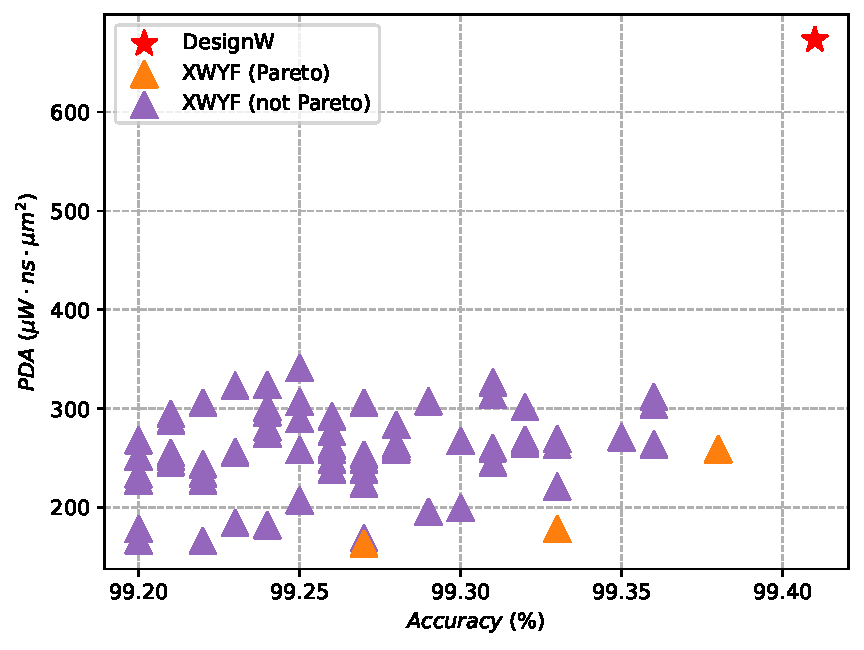
\includegraphics[width=\linewidth]{figs/LeNet_XWYF_PDA.pdf}
    \end{minipage}
    }
    \subfigure[基于XWYF实现的卷积加速器的评估结果]{
    \label{AC:ALS:Fig:SC}
    \begin{minipage}[t]{0.48\linewidth}
    \centering
    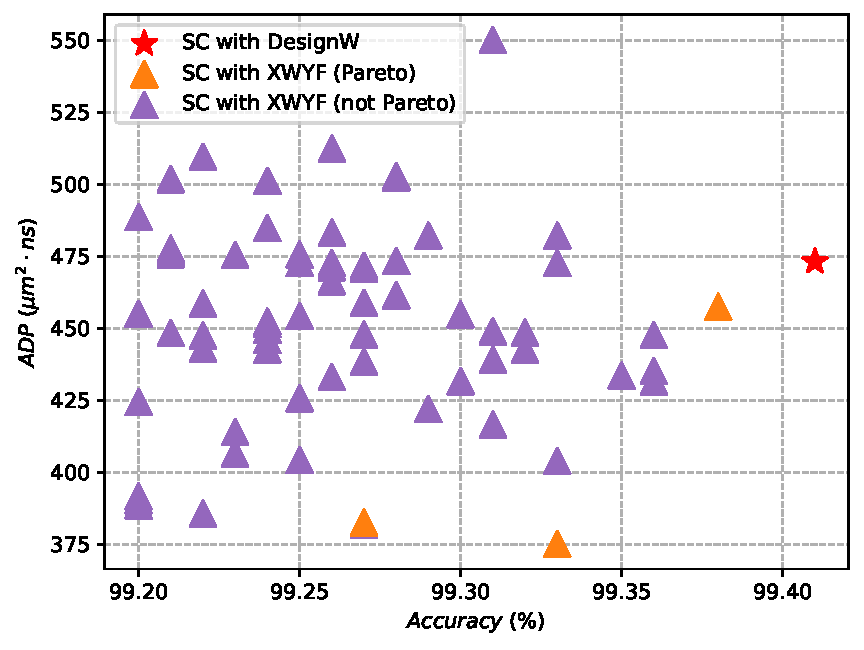
\includegraphics[width=\linewidth]{figs/SC_LeNet_XWYF_ADP.pdf}
    \end{minipage}
    }
\caption{XWYF乘法器的评估结果以及基于XWYF实现的卷积加速器的评估结果}
\label{AC:ALS:Fig:SC_LeNet_XWYF}
\end{figure}

图\ref{AC:ALS:Fig:SC_LeNet_XWYF}展示了68个XWYF乘法器的评估结果以及基于XWYF实现的68个卷积加速器SC\cite{Accelerator:SC}的评估结果,作为对比,基于DesignWare库\cite{IP:DesignWare}实现的精确乘法器DesignW也被纳入比较。图\ref{AC:ALS:Fig:LeNet_XWYF}中共有3个乘法器位于帕累拖前沿,以黄色三角形表示,对应的SC实现在图\ref{AC:ALS:Fig:SC}中也以黄色三角形表示。一个有意思的现象是,虽然DesignW的单独评估结果显示其PDA较高,但基于DesignW实现的SC模块的硬件开销却优于相当一部分的XWYF乘法器,这说明了近似乘法器库在使用时不能简单地根据单独的硬件成本直接选择,而是应该进行多次尝试后决定。
图\ref{AC:ALS:Fig:SC}表明,基于3个帕累拖最优的乘法器的SC实现仍然位于帕累拖前沿,因此当给定一个近似乘法器库进行综合时,可对库中位于帕累拖前沿的乘法器进行一定次数的随机搜索,综合比较后选择最好的那个进行实现。

\section{本章小结}

基于前面两种自动化方法得到的近似乘法器,本章利用强化学习方法对不同乘法器在大规模电路中的应用进行了近似逻辑综合的研究。
首先,本章介绍了基于MFFC自适应超图划分的端到端强化学习逻辑优化框架,该框架基于Yosys和ABC实现,首先利用Yosys对电路进行读入和解析,接着将电路中的组合逻辑提取出来并划分,划分完成后采用强化学习方法对所有的子电路并行地进行序列寻优,最后通过商业综合工具进行评估。基于超过150个电路的实验结果显示,与ABC的脚本resyn2相比,面积延迟积平均提高了5.17\%。
之后,本章将强化学习优化框架与基于数据分布和输入极性得到的近似乘法器库结合,对不同近似乘法器实现的DNN硬件加速器进行研究,结果显示乘法器和加速器之间的性能收益存在不匹配的现象,即乘法器本身的硬件开销低,基于该乘法器实现的DNN加速器的硬件开销不一定低。因此近似乘法器库在使用时不能简单地根据乘法器的单独硬件成本直接选择,而是应该进行多次尝试后决定。